\documentclass[bachelor, och, labwork]{shiza}

\usepackage{subfigure}
\usepackage{tikz,pgfplots}
\pgfplotsset{compat=1.5}
\usepackage{float}
\usepackage{pdfpages}

\usepackage{titlesec}
\setcounter{secnumdepth}{4}
\titleformat{\paragraph}
{\normalfont\normalsize}{\theparagraph}{1em}{}
\titlespacing*{\paragraph}
{35.5pt}{3.25ex plus 1ex minus .2ex}{1.5ex plus .2ex}

\titleformat{\paragraph}[block]
{\hspace{1.25cm}\normalfont}
{\theparagraph}{1ex}{}
\titlespacing{\paragraph}
{0cm}{2ex plus 1ex minus .2ex}{.4ex plus.2ex}

% --------------------------------------------------------------------------%

\usepackage{multirow}
\usepackage[T2A]{fontenc}
\usepackage[utf8]{inputenc}
\usepackage{graphicx}
\graphicspath{ {./images/} }
\usepackage{tempora}

\usepackage[sort,compress]{cite}
\usepackage{amsmath}
\usepackage{amssymb}
\usepackage{amsthm}
\usepackage{fancyvrb}
\usepackage{listings}
\usepackage{listingsutf8}
\usepackage{longtable}
\usepackage{array}
\usepackage[english,russian]{babel}

\usepackage[hidelinks]{hyperref}
\usepackage{url}

\usepackage{underscore}
\usepackage{setspace}
\usepackage{indentfirst} 
\usepackage{mathtools}
\usepackage{amsfonts}
\usepackage{enumitem}
\usepackage{tikz}
\usepackage{minted}

\newcommand{\eqdef}{\stackrel {\rm def}{=}}
\newcommand{\specialcell}[2][c]{%
\begin{tabular}[#1]{@{}c@{}}#2\end{tabular}}

\renewcommand\theFancyVerbLine{\small\arabic{FancyVerbLine}}


\begin{document}

\includepdf{titul.pdf}

%-------------------------------------------------------------------------------

\tableofcontents

\intro

В алгебрах могут быть заданы различные операции, которые могут иметь определенные
свойства: ассоциативность, коммутативность, идемпотентность, обратимость и
дистрибутивность относительно операции сложения.
Операции могут быть заданы с помощью матриц, при этом матрично можно проверить их
свойства. Существует понятие операций над бинарными отношениями. По определенным
алгоритмам можно производить ряд операций над матрицами: объединение, пересечение, 
инверсию, обращение и композицию. Также существуют как унарные (то есть операции, 
определенные для одной матрицы) и бинарные операции над матрицами отношений: сложение,
вычитание, произведение матрицы на константу, произведение двух матриц и транспонирование
матрицы.

\section{\textbf{Цель работы и порядок ее выполнения}}

\textbf{Цель работы} "--- изучение основных понятий универсальной алгебры и операций 
над бинарными отношениями.

Порядок выполнения работы:

\begin{enumerate}
    \item Рассмотреть понятие алгебраической операции и классификацию свойств операций. 
    Разработать алгоритмы проверки свойств операций: ассоциативность, коммутативность, 
    идемпотентность, обратимость, дистрибутивность.   

    \item Рассмотреть основные операции над бинарными отношениями. Разработать 
    алгоритмы выполнения операции над бинарными отношениями.  

    \item Рассмотреть основные операции над матрицами. Разработать алгоритмы 
    выполнения операций над матрицами.  
\end{enumerate}

\section{Теоретические сведения}

\subsection{Алгебраические операции}

Отображение $f:A^n\rightarrow A$ называется алгебраической n-арной операцией или
просто алгебраической операцией на множестве $A$. При этом n называется порядком
или арностью алгебраической операции $f$.

Далее для бинарной операции $f$ по возможности будем использовать мультипликативную
запись с помощью символа $\cdot$, то есть вместо $f(x,y)$ писать $x\cdot y$.

\subsubsection{Свойства алгебраических операций}
Бинарная операция $\cdot$ на множестве $A$ называется:
\begin{enumerate}
    \item \textit{ассоциативной}, если $\forall x,y,z \in A ~\text{выполняется}~ x\cdot (y\cdot z) = (x\cdot y)\cdot z$,
    \item \textit{коммутативной}, если $\forall x,a \in A ~\text{выполняется}~ x\cdot y = y\cdot x$,
    \item \textit{идемпотентной}, если $\forall x \in A$ выполняется $x\cdot x=x$,
    \item \textit{обратимой}, если $\forall x \in A ~\exists a: x\cdot a = a\cdot x = 1$,
    \item \textit{дистрибутивной относительно операции +}, если $\forall x,y,z \in A$
    выполняются равенства $x\cdot (y+z)=(x\cdot y)+(x\cdot z),~ (y+z)\cdot x=(y\cdot x)+(z\cdot x)$.
\end{enumerate}

\subsubsection{Алгоритм проверки операции на ассоциативность}

\textit{Вход}: Таблица Кэли операции $A=(a_{ij})$, размерности $n\times n$ и
множество $S$ размерности $n$, на котором задана операция.

\textit{Выход}: <<Операция является ассоциативной>> или <<Операция не является
ассоциативной>>.

\begin{enumerate}
    \item Цикл по $i$ от 1 до $n$.
        \begin{enumerate}
            \item Создать пустое множество $S_1$.
            \item Цикл по $j$ от 1 до $n$.
            \begin{enumerate}
                \item Добавить в $S_1$ значение $a[i][j]$.
            \end{enumerate}
            \item Создать пустое множество $A_1$ размерности $n\times n$ для таблицы Кэли.
            \item Цикл по $j$ от 1 до $n$, цикл по $k$ от 1 до $n$.
            \begin{enumerate}
                \item Создать переменную $ind$ и присвоить ей значение индекса
                $S_1[k]$ в множестве $S$.
                \item Присвоить $A_1[j][k]$ значение $a[j][ind]$.
            \end{enumerate}
            \item Создать пустое множество $S_2$.
            \item Цикл по $j$ от 1 до $n$.
            \begin{enumerate}
                \item Добавить в $S_2$ значение $a[j][i]$.
            \end{enumerate}
            \item Создать пустое множество $A_2$ размерности $n\times n$ для таблицы Кэли.
            \item Цикл по $j$ от 1 до $n$, цикл по $k$ от 1 до $n$.
            \begin{enumerate}
                \item Создать переменную $ind$ и присвоить ей значение индекса
                $S_1[j]$ в множестве $S$.
                \item Присвоить $A_2[j][k]$ значение $a[ind][k]$.
            \end{enumerate}
            \item Цикл по $j$ от 1 до $n$, цикл по $k$ от 1 до $n$.
            \begin{enumerate}
                \item Если $A_1[j][k]\not=A_2[j][k]$, то ответ --- <<Операция не 
                является ассоциативной>>.
            \end{enumerate}
        \end{enumerate}
    \item Ответ --- <<Операция является ассоциативной>>.
\end{enumerate}

Трудоемкость алгоритма $O(N^3)$.

\subsubsection{Алгоритм проверки операции на коммутативность}

\textit{Вход}: Таблица Кэли операции $A=(a_{ij})$, размерности $n\times n$.

\textit{Выход}: <<Операция является коммутативной>> или <<Операция не является
коммутативной>>.

\begin{enumerate}
    \item Цикл по $i$ от 1 до $n$, цикл по $j$ от 1 до $n$.
        \begin{enumerate}
            \item Если $a_{ij} \not = a_{ji}$, то ответ --- <<Операция не
            является коммутативной>>.
        \end{enumerate}
    \item Ответ --- <<Операция является коммутативной>>.
\end{enumerate}

Трудоемкость алгоритма $O(N^2)$.

\subsubsection{Алгоритм проверки операции на идемпотентность}

\textit{Вход}: Таблица Кэли операции $A=(a_{ij})$, размерности $n\times n$ и
множество $S$ размерности $n$, на котором задана операция.

\textit{Выход}: <<Операция является идемпотентной>> или <<Операция не является
идемпотентной>>.

\begin{enumerate}
    \item Цикл по $i$ от 1 до $n$.
        \begin{enumerate}
            \item Если $a[i][i] \not= s[i]$, то ответ --- <<Операция не является
            идемпотентной>>.
        \end{enumerate}
    \item Ответ --- <<Операция является идемпотентной>>.
\end{enumerate}

Трудоемкость алгоритма $O(N)$.

\subsubsection{Алгоритм проверки операции на обратимость}

\textit{Вход}: Таблица Кэли операции $A=(a_{ij})$, размерности $n\times n$ и
множество $S$ размерности $n$, на котором задана операция.

\textit{Выход}: <<Список обратных элементов матрицы $B$>> или <<Операция не является
обратимой>>.

\begin{enumerate}
    \item Создать пустое множество $B$.
    \item Цикл по $i$ от 1 до $n$, цикл по $j$ от 1 до $n$.
        \begin{enumerate}
            \item Если $a[i][j] = a[j][i] = 1$, то добавить $S[i]$ во множество
            $B$.
        \end{enumerate}
    \item Если полученное множество $B$ непустое, то ответ --- <<Список обратных 
    элементов матрицы $B$>>, если же множество $B$ пустое, то ответ --- <<Операция 
    не является обратимой>>.
\end{enumerate}

Трудоемкость алгоритма $O(N^2)$.

\subsubsection{Алгоритм проверки операции на дистрибутивность}

\textit{Вход}: таблица Кэли операции * $A = (a_{ij})$, размерности $n \times n$, 
таблица Кэли операции + $A' = (a'_{ij})$, относительно которой делается проверка 
на дистрибутивность, размерности $n \times n$, множество элементов $S$, размерности 
$n$, на котором заданы обе операции.

\textit{Выход}: <<Операция * является дистрибутивной относительно операции +>> или 
<<Операция * не является дистрибутивной относительно операции +>>.

\begin{enumerate}
    \item Цикл по $i$ от 1 до $n$, цикл по $j$ от 1 до $n$, цикл по $k$ от 1 до $n$.
        \begin{enumerate}
            \item Создать переменную $d = ~\text{индекс}~a^{'}[j][k]$ во
            множестве $S$.
            \item Создать переменную $v = ~\text{индекс}~a[i][j]$ во
            множестве $S$.
            \item Создать переменную $h = ~\text{индекс}~a[i][k]$ во
            множестве $S$.
            \item Создать переменную $f = ~\text{индекс}~a^{'}[j][k]$
            \item Создать переменную $k = ~\text{индекс}~a[k][i]$ во
            множестве $S$.
            \item Если $a[i][d] \not= a'[v][h]$ или $a[f][i] \not= a'[t][k]$, то 
            ответ --- <<Операция * не является дистрибутивной относительно операции +>>.
        \end{enumerate}
    \item Ответ --- <<Операция * является дистрибутивной относительно операции +>>.
\end{enumerate}

Трудоемкость алгоритма $O(N^3)$.

\subsection{Основные операции над бинарными отношениями}
\begin{enumerate}
    \item Теоретико-множественные операции ($\cup,\cap, \neg$).
    \item Обращение бинарных отношений: \textit{обратным} для бинарного отношения
    $\rho \subset A\times B$ называется бинарное отношение $\rho^{-1} \subset B \times A$,
    определяемое по формуле: $\rho^{-1}=\{(b,a):(a,b)\in\rho\}.$
    \item Композиция бинарных отношений: \textit{композицией} бинарных отношений
    $\rho\subset A\times B$ и $\sigma\subset B\times C$ называется бинарное
    отношение $\rho\sigma=\{(a,c):(a,b)\in\rho$ и $(b,c)\in\sigma ~\text{для некоторого}~ b \in B\}$.
    Если бинарное отношение $A=(a_{ij})$ размерности $n\times m$ и 
    бинарное отношение $B=(b_{ij})$ размерности $m\times h$, то бинарное отношение
    композиции этих отношений будет иметь размерность $n \times h$.
\end{enumerate}

\subsubsection{Алгоритм построения объединения бинарных отношений}

\textit{Вход}: бинарное отношение $A=(a_{ij})$ размерности $n\times m$ и 
бинарное отношение $B=(b_{ij})$ размерности $n\times m$.

\textit{Выход}: бинарное отношение $C=(c_{ij})$ размерности $n\times m$ объединения
бинарных отношений $A$ и $B$.

\begin{enumerate}
    \item Создать матрицу $C$ размерности $n\times m$ и заполнить ее нулями.
    \item Цикл по $i$ от 1 до $n$, цикл по $j$ от 1 до $m$.
    \begin{enumerate}
        \item $c[i][j]$ присвоить значение $a[i][j] \vee b[i][j]$.
    \end{enumerate}
    \item Ответ --- бинарное отношение $C=(c_{ij})$ размерности $n\times m$ объединения
    бинарных отношений $A$ и $B$.
\end{enumerate}

Трудоемкость алгоритма $O(N^2)$.

\subsubsection{Алгоритм построения пересечения бинарных отношений}

\textit{Вход}: бинарное отношение $A=(a_{ij})$ размерности $n\times m$ и 
бинарное отношение $B=(b_{ij})$ размерности $n\times m$.

\textit{Выход}: бинарное отношение $C=(c_{ij})$ размерности $n\times m$ пересечения
бинарных отношений $A$ и $B$.

\begin{enumerate}
    \item Создать матрицу $C$ размерности $n\times m$ и заполнить ее нулями.
    \item Цикл по $i$ от 1 до $n$, цикл по $j$ от 1 до $m$.
    \begin{enumerate}
        \item $c[i][j]$ присвоить значение $a[i][j] \wedge b[i][j]$.
    \end{enumerate}
    \item Ответ --- бинарное отношение $C=(c_{ij})$ размерности $n\times m$ объединения
    бинарных отношений $A$ и $B$.
\end{enumerate}

Трудоемкость алгоритма $O(N^2)$.

\subsubsection{Алгоритм построения дополнения бинарного отношения}

\textit{Вход}: бинарное отношение $A=(a_{ij})$ размерности $n\times m$.

\textit{Выход}: бинарное отношение $B=(b_{ij})$ размерности $n\times m$ дополения
бинарного отношения $A$.

\begin{enumerate}
    \item Создать матрицу $B$ размерности $n\times n$ и заполнить ее нулями.
    \item Цикл по $i$ от 1 до $n$, цикл по $j$ от 1 до $m$.
    \begin{enumerate}
        \item $b[i][j]$ присвоить значение $\neg a[i][j]$ (то есть если значение
        $a[i][j]$ было равно единице, то $b[i][j]$ присвоится значение 0, если
        же значение $a[i][j]$ было равно нулю, то $b[i][j]$ присвоится значение 1).
    \end{enumerate}
    \item Ответ --- бинарное отношение $B=(b_{ij})$ размерности $n\times m$ дополнения
    бинарного отношения $A$.
\end{enumerate}

Трудоемкость алгоритма $O(N^2)$.

\subsubsection{Алгоритм построения композиции бинарных отношений}

\textit{Вход}: бинарное отношение $A=(a_{ij})$ размерности $n\times m$ и
бинарное отношение $B=(b_{ij})$ размерности $m\times h$.

\textit{Выход}: бинарное отношение $C=(c_{ij})$ размерности $n\times h$ композиции
бинарных отношений $A$ и $B$.

\begin{enumerate}
    \item Создать матрицу $C$ размерности $n\times h$ и заполнить ее нулями.
    \item Цикл по $i$ от 1 до $n$, цикл по $j$ от 1 до $n$.
    \begin{enumerate}
        \item с[i][j] присвоить $sgn(\sum_{p = 1}^{n}a[i][p]b[p][j])$, где $sgn$
        --- знак полученного числа: если число > 0, то значение функции станет равно
        1, если число <= 0, то значение функции станет равно 0.
    \end{enumerate}
    \item Ответ --- бинарное отношение $C=(c_{ij})$ размерности $n\times h$ композиции
    бинарных отношений $A$ и $B$.
\end{enumerate}

Трудоемкость алгоритма $O(n \times m \times h)$.

\subsection{Основные операции над матрицами}
\subsubsection{Сложение и вычитание матриц}
Суммой $A+B$ матриц $A_{n\times m}=(a_{ij})$ и $B_{n\times m}=(b_{ij})$ называется
матрица $C_{n\times m}=(c_{ij})$, где $(c_{ij})=(a_{ij})+(b_{ij})$ для всех $i=\overline{1,n}$
и $j=\overline{1,m}$.

\subsubsection{Алгоритм сложения матриц}

\textit{Вход}: Матрица $A=(a_{ij})$ размерности $n\times m$ и
матрица $B=(b_{ij})$ размерности $n\times m$, характеристика поля $X$.

\textit{Выход}: Матрица $C=(c_{ij})$ размерности $n\times m$ суммы 
матриц $A$ и $B$.

\begin{enumerate}
    \item Создать матрицу $C$ размерности $n\times m$ и заполнить ее нулями.
    \item Цикл по $i$ от 1 до $n$, цикл по $j$ от 1 до $m$.
    \begin{enumerate}
        \item $c[i][j]$ присвоить значение $(a[i][j] + b[i][j]) ~mod~ X$.
    \end{enumerate}
    \item Ответ --- матрица $C=(c_{ij})$ размерности $n\times m$ суммы матриц $A$ и $B$.
\end{enumerate}

Трудоемкость алгоритма $O(n \times m)$.

Разностью $A-B$ матриц $A_{n\times m}=(a_{ij})$ и $B_{n\times m}=(b_{ij})$ называется
матрица $C_{n\times m}=(c_{ij})$, где $(c_{ij})=(a_{ij})-(b_{ij})$ для всех $i=\overline{1,n}$
и $j=\overline{1,m}$.

\subsubsection{Алгоритм вычитания матриц}

\textit{Вход}: Матрица $A=(a_{ij})$ размерности $n\times m$ и
матрица $B=(b_{ij})$ размерности $n\times m$, характеристика поля $X$.

\textit{Выход}: Матрица $C=(c_{ij})$ размерности $n\times m$ разности 
матриц $A$ и $B$.

\begin{enumerate}
    \item Создать матрицу $C$ размерности $n\times m$ и заполнить ее нулями.
    \item Цикл по $i$ от 1 до $n$, цикл по $j$ от 1 до $m$.
    \begin{enumerate}
        \item $c[i][j]$ присвоить значение $(a[i][j] - b[i][j]) ~mod~ X$.
    \end{enumerate}
    \item Ответ --- матрица $C=(c_{ij})$ размерности $n\times m$ разности матриц $A$ и $B$.
\end{enumerate}

Трудоемкость алгоритма $O(n \times m)$.

\subsubsection{Умножение матрицы на число}

Произведением матрицы $A_{n\times m}=(a_{ij})$ на число $\alpha$ называется матрица
$C_{n\times m}=(c_{ij})$, где $c_{ij}=\alpha a_{ij}$ для всех $i=\overline{1,n}$
и $j=\overline{1,m}$.

\subsubsection{Алгоритм умножения матрицы на число}

\textit{Вход}: Матрица $A=(a_{ij})$ размерности $n\times m$, число $\alpha$, характеристика поля $X$.

\textit{Выход}: Матрица $C=(c_{ij})$ размерности $n\times m$ умноженной на число 
$\alpha$ матрицы $A$.

\begin{enumerate}
    \item Создать матрицу $C$ размерности $n\times m$ и заполнить ее нулями.
    \item Цикл по $i$ от 1 до $n$, цикл по $j$ от 1 до $m$.
    \begin{enumerate}
        \item $c[i][j]$ присвоить значение $\alpha a[i][j] ~mod~ X$.
    \end{enumerate}
    \item Ответ --- матрица $C=(c_{ij})$ размерности $n\times m$ умноженной на число 
    $\alpha$ матрицы $A$.
\end{enumerate}

Трудоемкость алгоритма $O(n \times m)$.

\subsubsection{Произведение двух матриц}

Произведением матрицы $A_{m\times n}=(a_{ij})$ на матрицу $B_{m\times p}=(b_{ij})$
называется матрица $C_{m\times p}=(c_{ij})$, где $c_{ij}=\sum_{p = 1}^{n}a_{ip}b_{pj}$
для всех $i=\overline{1,m}$ и $j= \overline{1,n}$.

\subsubsection{Алгоритм умножения матриц}

\textit{Вход}: Матрица $A=(a_{ij})$ размерности $n\times m$ и
матрица $B=(b_{ij})$ размерности $p\times n$, характеристика поля $X$.

\textit{Выход}: Матрица $C=(c_{ij})$ размерности $n\times p$ умножения
матрицы $A$ на матрицу $B$.

\begin{enumerate}
    \item Создать матрицу $C$ размерности $n\times p$ и заполнить ее нулями.
    \item Цикл по $i$ от 1 до $n$, цикл по $j$ от 1 до $m$.
    \begin{enumerate}
        \item Создать переменную $cur$ и присвоить ей значение ноль.
        \item Цикл по $p$ от 1 до $n$
        \begin{enumerate}
            \item Переменной $cur$ присвоить значение $(cur + a[i][p]b[p][j]) ~mod~ X$.
        \end{enumerate}
    \end{enumerate}

    \item Ответ --- матрица $C=(c_{ij})$ размерности $n\times p$ умножения матрицы   
    $A$ на матрицу $B$.
\end{enumerate}

Трудоемкость алгоритма $O(n \times m \times p)$.

\subsubsection{Транспорирование матрицы}
Транспонированной по отношению к матрице $A_{m\times n}=(a_{ij})$ называется матрица
$A^T_{n\times m}=(a^T_{ij})$ для элементов которой $a^T_{ij}=a_{ji}.$

\textit{Вход} Матрица $A = (a_{ij})$ размерности $n \times m$.\\

\textit{Выход} Матрица $A^T = A' = (a'_{ij})$.\\

\begin{enumerate}
    \item Создать матрицу $C$ размерности $m\times n$ и заполнить ее нулями.
    \item Цикл по $i$ от 1 до $n$, цикл по $j$ от 1 до $m$.
    \begin{enumerate}
        \item с[j][i] присвоить $a[i][j]$.
    \end{enumerate}
    \item Ответ --- матрица $C=(c_{ij})$ размерности $m\times n$ транспонированной матрицы $A$.
\end{enumerate}

Трудоемкость алгоритма $O(n \times m)$.

\subsubsection{Обращение матрицы}

Обращенной по отношения к матрице  $A_{n\times n}=(a_{ij})$ называется матрица 
$A^{-1}_{n\times n}=(a^{-1}_{ij})$, при умножении которой на исходную матрицу 
$A$ получается единичная матрица $E$: $AA^{-1}=A^{-1}A=E$.

\subsubsection{Алгоритм нахождения обратной матрицы в конечном поле}

\begin{center}
    \textit{Алгоритм нахождения минора}
\end{center}

Пусть функция нахождения минора матрицы будет называться $get\_minor$

\textit{Вход} Матрица $A = (a_{ij})$ размерности $n \times n$, номер столбца $column$.

\textit{Выход} Минор матрицы $A = (a_{ij})$ относительно столбца $column$.\\

\begin{enumerate}
    \item Создать пустой список $minor$ для хранения миноров матрицы.
    \item Цикл по $i$ от 1 до $n$.
    \begin{enumerate}
        \item Создать пустой список $row$.
        \item Цикл по $j$ от 1 до $n$.
        \begin{enumerate}
            \item Если $j \not = column$, добавить $a[i][j]$ в список $row$.
        \end{enumerate}
        \item Добавить список $row$ в список $minor$
    \end{enumerate}
    \item Ответ --- минор матрицы $A=(a_{ij})$.
\end{enumerate}

Трудоемкость алгоритма $O(n \times n)$.

\begin{center}
    \textit{Алгоритм нахождения определителя матрицы}
\end{center}

Пусть функция нахождения определителя матрицы будет называться $get\_det$

\textit{Вход} Матрица $A = (a_{ij})$ размерности $n \times n$.

\textit{Выход} Определитель матрицы $A$.

\begin{enumerate}
    \item Если размер матрицы равен единице, то ответ --- $a[0][0]$.
    \item Создать переменную $det=0$.
    \item Создать переменную $multiplier=1$.
    \item Цикл по $i$ от 1 до $n$.
        \begin{enumerate}
            \item Создать переменную $el=a[0][i]$.
            \item Если $el \not = 0$, то переменной $det$ присвоить значение
            $det + multiplier * el * get\_det(get\_minor(i, A))$.
            \item Переменной $multiplier$ присвоить значение $multiplier * -1$
        \end{enumerate}
    \item Ответ --- определитель матрицы $A=(a_{ij})$.
\end{enumerate}

Трудоемкость алгоритма $O(\frac{(n + 1)\times n }{2} \times n \times n)$, так как сложность алгоритма нахождения 
минора составляет $O(n \times n)$ и внутри алгоритма нахождения определителя происходит
обращение к данному алгоритму $O(\frac{(n + 1)\times n}{2})$

\begin{center}
    \textit{Алгоритм нахождения обратного по модулю элемента}
\end{center}


Модульное обратное для числа $a$ по модулю $m$ можно найти с помощью расширенного 
алгоритма Евклида.

Алгоритм Евклида определяет наибольший общий делитель (НОД) двух целых чисел, скажем $a$ и $m$. 
Если $a$ имеет обратное по модулю $m$ число, этот НОД должен быть равен 1. Несколько 
последних равенств, получаемых в процессе работы алгоритма, могут быть решены для 
нахождения НОД. Затем, используя метод <<обратной подстановки>>, может быть получено 
выражение, связывающее исходные параметры и НОД. Другими словами, могут быть 
найдены целые $x$ и $y$, удовлетворяющие равенство Безу:
\begin{center}
    $\alpha x + my = \text{НОД}(\alpha, m) = 1$
\end{center}

Данное равенство можно переписать следующим образом:

\begin{center}
    $\alpha x - 1= (-y)m$, то есть $\alpha x \equiv 1 ~~(mod ~m )$ и модульное обратное числа a вычислено.
\end{center}

Более эффективной версией является расширенный алгоритм Евклида, который с помощью 
дополнительных равенств сокращает два прохода алгоритма (обратную подстановку можно 
понимать как прохождение алгоритма в обратном порядке) до одного.

Сложность алгоритма составляет $O(log(m)^2)$ из условия, что $| \alpha \vert < m$.

Пусть функция нахождения обратного по модулю будет называться $get\_extended$

\textit{Вход} Число $x$, число $y$, обратный определитель матрицы $A = (a_{ij})$ $detInverse$,
модуль $FieldOrder$, определитель $a$ матрицы $A = (a_{ij})$, вспомогательная переменная $b$, 
изначально равная $FieldOrder$.

\textit{Выход} Обратный по модулю $FieldOrder$ элемент.

\begin{enumerate}
    \item Если $a=0$, то ответ --- 0.
    \item Создать переменную $y\_1=0$.
    \item Создать переменную $x\_1=0$.
    \item Переменной $FieldOrder$ присвоить значение $a$.
    \item Переменной $a$ присвоить значение $b ~mod~ a$
    \item Вызвать функцию $get\_extended$.
    \item Переменной $x$ присвоить значение $y\_1 - (\frac{b}{a} * x\_1)$.
    \item Переменной $y\_1$ присвоить значение $x_1$.
    \item Ответ --- обратный по модулю $FieldOrder$ элемент.
\end{enumerate}

Трудоемкость алгоритма составляет $O(log(m)^2) = O(log(m))$.

\begin{center}
    \textit{Алгоритм нахождения расширенного минора матрицы}
\end{center}

Пусть функция нахождения расширенного минора матрицы будет называться $get\_minor\_extended$.

\textit{Вход} Матрица $A = (a_{ij})$ размерности $n \times n$, столбец $column$, 
строка $row$.

\textit{Выход} Расширенный минор матрицы $A$ по строке $row$ и столбцу $column$.

\begin{enumerate}
    \item Создать пустой список $minor$.
    \item Цикл по $i$ от 1 до $n$.
        \begin{enumerate}
            \item Если $i = row$, перейти к следующей итерации.
            \item Создать пустой список $row\_temp$.
            \item Цикл по $j$ от 1 до $n$.
                \begin{enumerate}
                    \item Если $j=column$, перейти к следующей итерации.
                    \item Добавить в $row\_temp$ элемент $a[i][j]$.
                \end{enumerate}
            \item Добавить в список $minor$ список $row\_temp$.
        \end{enumerate}
    \item Ответ --- расширенный минор матрицы $A$ по строке $row$ и столбцу $column$.
\end{enumerate}

Трудоемкость алгоритма $O(n \times n)$.

\begin{center}
    \textit{Алгоритм нахождения сопряженной матрицы}
\end{center}

\textit{Вход} Матрица $A = (a_{ij})$ размерности $n \times n$.

\textit{Выход} Сопряженная матрица матрице $A$.

\begin{enumerate}
    \item Создать переменную $sign=1$.
    \item Создать переменную $flag$ и присвоить ей значение 1, если размерность 
    матрицы четная. Если размерность матрицы нечетная, то присвоить переменной $flag$
    значение 0.
    \item Создать матрицу $con\_matrix$ размерности $n \times n$
    и заполнить ее нулями.
    \item Цикл по $i$ от 1 до $n$, цикл по $j$ от 1 до $n$.
        \begin{enumerate}
            \item $con\_matrix[i][j]$ присвоить значение $sign * get\_det(get\_minor\_extended(A, i, j))$.
            \item Переменной $sign$ присвоить значение $sign * (-1)$
            \item Перед каждой новой итерацией по $i$ присваивать $sign$ значение $sign * (-1)$, 
            если $flag = 1$.
        \end{enumerate}
    \item Вызвать алгоритм транспонирования матрицы от полученной матрицы $con_matrix$.

    \item Ответ --- сопряженная матрица матрице $A$.
\end{enumerate}

Внутри алгоритма нахождения сопряженной матрицы $n \times n$ раз вызывается алгоритм 
нахождения определителя $O(\frac{(n + 1)\times n }{2})$, а также алгоритм нахождения расширенного 
минора матрицы $O(n \times n)$, затем вызывается алгоритм получения транспонированной 
матрицы, сложность которого составляет $O(n \times n)$. Поэтому, трудоемкость алгоритма
составляет $O(n \times n \times n \times n \times \frac{(n + 1)\times n }{2} + n \times n) = O(\frac{(n + 1)\times n^5}{2} + n \times n) = O(n ^ 6)$.


\begin{center}
    \textit{Алгоритм свертки матрицы по модулю}
\end{center}


\textit{Вход} Матрица $A = (a_{ij})$ размерности $n \times n$, обратный определитель
матрицы $detInverse$, модуль $FieldOrder$.

\textit{Выход} Обратная матрица к матрице $A$.

\begin{enumerate}
    \item Создать матрицу $A_1 = (a_{1_{ij}})$ размерности $n \times n$ и заполнить
    ее нулями
    \item Цикл по $i$ от 1 до $n$, цикл по $j$ от 1 до $n$.
        \begin{enumerate}
            \item Элементу $a_1[i][j]$ присвоить значение $(a[i][j] * detInverse) mod FieldOrder$.
            \item Если $a_1[i][j] < 0$, то $a_1[i][j]$ присвоить значение $a_1[i][j] + FieldOrder$
            \item Перед каждой новой итерацией по $i$ присваивать $sign$ значение $sign * (-1)$, 
            если $flag = 1$.
        \end{enumerate}
    \item Ответ --- обратная матрица матрице $A$.
\end{enumerate}

Трудоемкость алгоритма составляет $O(n \times n)$.

% \section{Практическая часть}\nopagebreak

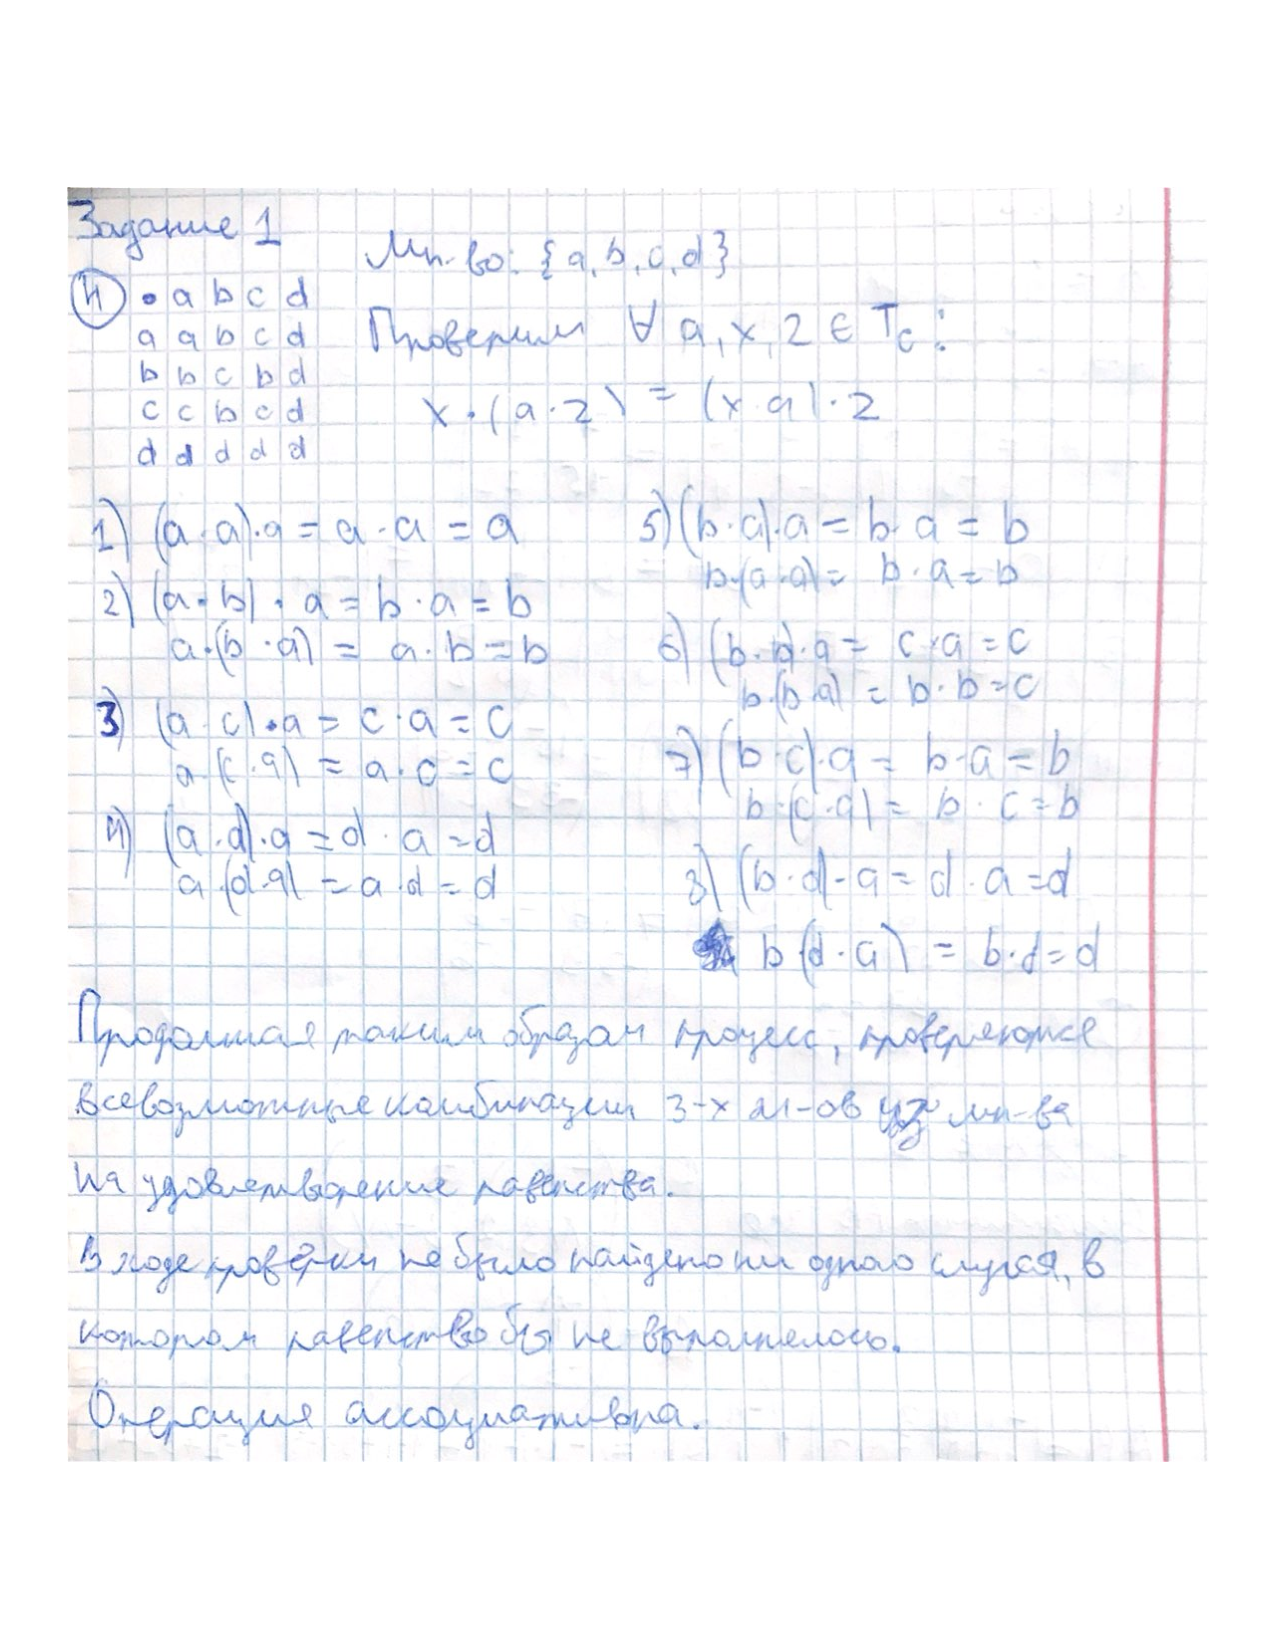
\includepdf[pages={1}, pagecommand=\section{Практическая часть}]{Zad3lab.pdf}
\includepdf[pages={2}]{Zad3lab.pdf}
\section{Программная реализация рассмотренных алгоритмов}
    
    \subsection{Результаты тестирования программы}

        \begin{figure}[H]
            \centering
            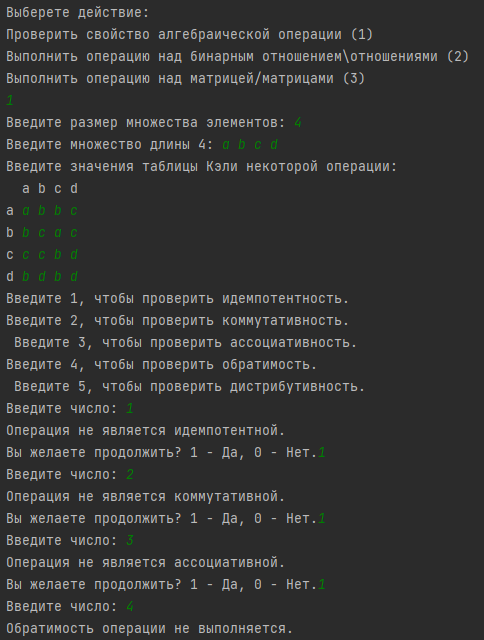
\includegraphics[width=0.8\textwidth]{pic/1.png}
            \caption{}
        \end{figure}

        \begin{figure}[H]
            \centering
            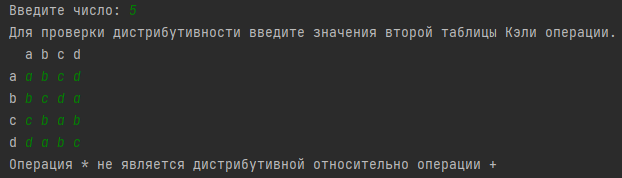
\includegraphics[width=0.8\textwidth]{pic/2.png}
            \caption{}
        \end{figure}

        \begin{figure}[H]
            \centering
            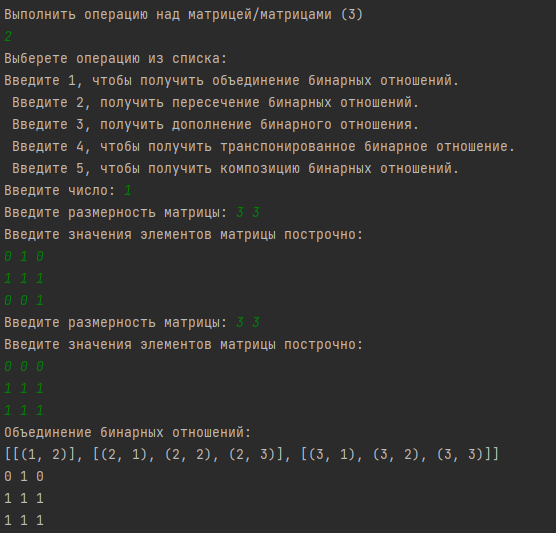
\includegraphics[width=0.8\textwidth]{pic/3.png}
            \caption{}
        \end{figure}

        \begin{figure}[H]
            \centering
            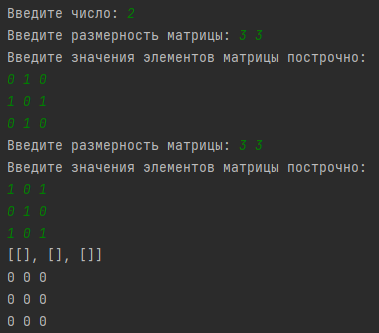
\includegraphics[width=0.8\textwidth]{pic/4.png}
            \caption{}
        \end{figure}

        \begin{figure}[H]
            \centering
            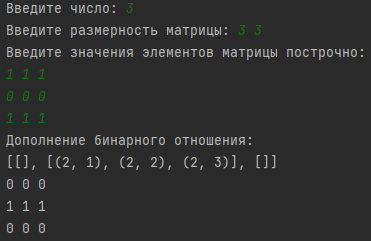
\includegraphics[width=0.8\textwidth]{pic/5.png}
            \caption{}
        \end{figure}

        \begin{figure}[H]
            \centering
            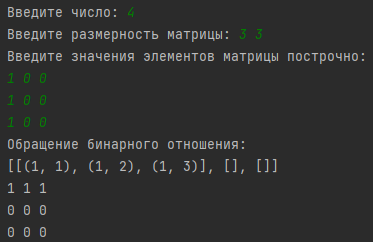
\includegraphics[width=0.8\textwidth]{pic/6.png}
            \caption{}
        \end{figure}

        \begin{figure}[H]
            \centering
            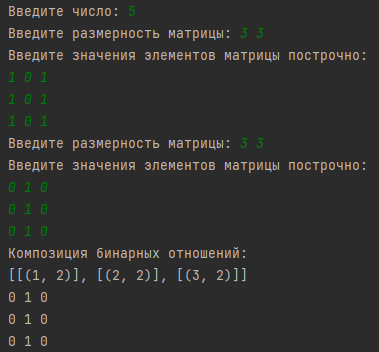
\includegraphics[width=0.8\textwidth]{pic/7.png}
            \caption{}
        \end{figure}

        \begin{figure}[H]
            \centering
            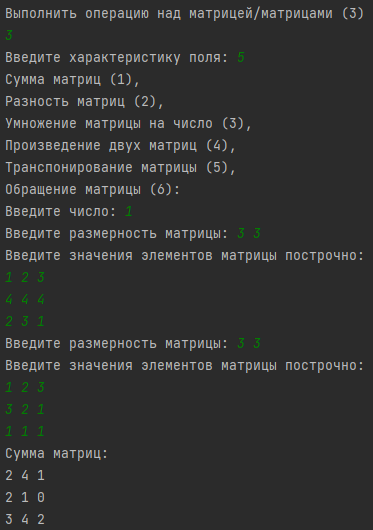
\includegraphics[width=0.8\textwidth]{pic/8.png}
            \caption{}
        \end{figure}

        \begin{figure}[H]
            \centering
            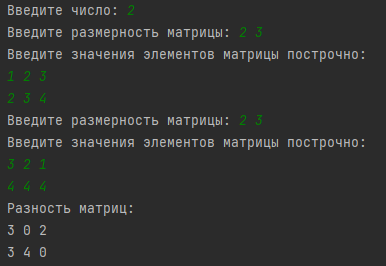
\includegraphics[width=0.8\textwidth]{pic/9.png}
            \caption{}
        \end{figure}

        \begin{figure}[H]
            \centering
            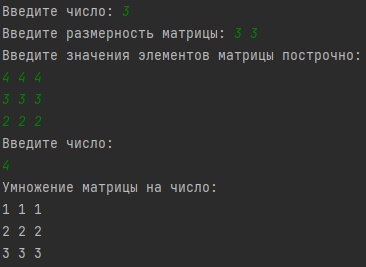
\includegraphics[width=0.8\textwidth]{pic/10.png}
            \caption{}
        \end{figure}

        \begin{figure}[H]
            \centering
            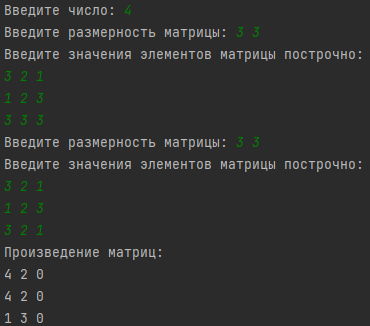
\includegraphics[width=0.8\textwidth]{pic/11.png}
            \caption{}
        \end{figure}

        \begin{figure}[H]
            \centering
            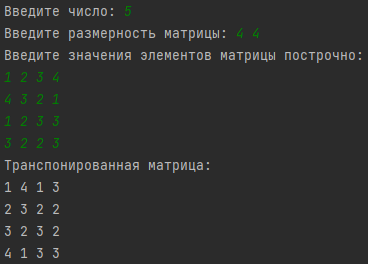
\includegraphics[width=0.8\textwidth]{pic/12.png}
            \caption{}
        \end{figure}

        \begin{figure}[H]
            \centering
            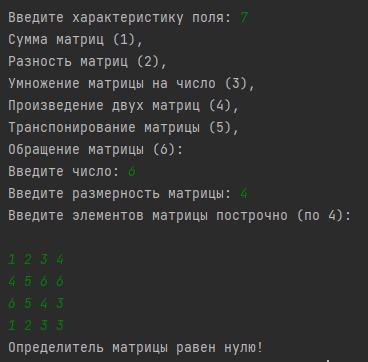
\includegraphics[width=0.8\textwidth]{pic/13.png}
            \caption{}
        \end{figure}
        
    \subsection{Коды программ, реализующих рассмотренные алгоритмы}
    \setminted[python]{linenos,breaklines=true, fontsize=\small, style=bw}
        \subsubsection{Код программы, реализующей нахождение обратной матрицы в поле Галуа}
            \inputminted{python}{code/inverseMatrix.py}
        \subsubsection{Код программы, реализующей основные алгоритмы}
            \inputminted{python}{code/lab3.py}
      


\conclusion
В ходе лабораторной работы были теоретические сведения об алгебраической операции 
и классификации свойств операций, основные операции над бинарными отношениями, а 
также основные операции над матрицами. На их основе были составлены алгоритмы проверки 
свойств операций: ассоциативность, коммутативность, идемпотентность, обратимость,
дистрибутивность, алгоритмы выполнения операции над бинарными отношениями, а также 
алгоритмы выполнения операций над матрицами. Для всех алгоритмов произведена 
асимптотическая оценка.
\end{document}